\chapter{从路径积分到传播子和顶点}

在转向粒子及其相互作用的清单之前，值得把核心构造讲清楚。拉格朗日量不仅仅编码经典场方程。通过路径积分，它还给出粒子传播、分裂、合并和散射的振幅。这是从量子场论通向费曼图的最直接途径。

\section{粒子与场的最小作用量原理}

费曼路径积分是最小作用量原理的量子对应物。从普通的牛顿粒子开始，其拉格朗日量依赖于坐标和速度，
\begin{equation}
\mathcal{L}=\mathcal{L}(x,\dot{x}),
\end{equation}
而赋予一条轨迹的作用量为
\begin{equation}
S[x]=\int \mathcal{L}(x,\dot{x})\,dt.
\end{equation}
从一个时空点到另一个时空点的每一条候选轨迹都有一个作用量，无论它是否满足牛顿方程。经典轨迹以作用量取驻值为标志。在传统的``最小作用量''表述中，它使作用量取极小值，不过取驻值是更一般的说法。驻值条件给出经典的微分运动方程。

\begin{figure}[htbp]
\centering
\includegraphics[width=0.72\textwidth]{lecture_10_figure_02.png}
\caption{粒子轨迹的作用量积分。}
\lectureframe{00:02:14}
\end{figure}

同样的结构适用于经典场。把所有场统记为\(\phi\)。局域场拉格朗日密度可以依赖于场以及场的空间和时间导数：
\begin{equation}
\mathcal{L}
=\mathcal{L}\!\left(\phi,\frac{\partial\phi}{\partial x^\mu}\right)
=\mathcal{L}(\phi,\partial_\mu\phi).
\end{equation}
相对论要求\(\mathcal{L}\)按洛伦兹标量变换。在这一要求下，由场及其导数构成的标量组合提供了拉格朗日量中可能的项。

\begin{figure}[htbp]
\centering
\includegraphics[width=0.62\textwidth]{lecture_10_figure_03.png}
\caption{场拉格朗日量对场及其时空导数的依赖关系。}
\lectureframe{00:04:09}
\end{figure}

对于场，作用量在时空的某个区域上积分：
\begin{equation}
S[\phi]=\int_{\Omega} d^4x\,\mathcal{L}(\phi,\partial_\mu\phi),
\qquad
d^4x=dt\,dx\,dy\,dz.
\end{equation}
粒子作用量是沿一条路径对时间的积分。场作用量则是在一个时空区域上对拉格朗日密度的积分。

固定粒子路径端点的类比，是在初始时间切片和最终时间切片上给定完整的场位形。如果初始场为\(\phi_{\mathrm{i}}(\mathbf{x})\)，最终场为\(\phi_{\mathrm{f}}(\mathbf{x})\)，则一个插值场填满二者之间的整个板状区域。当边界数据允许存在经典插值解时，该解就是在边界位形固定下作用量的驻点。
\editorialnote{两个时间切片上任意完整的场位形未必允许经典解。因此，驻值作用量的陈述仅限于存在插值解的边界数据。}

这一几何结构是粒子路径在场论中的对应物。\footnote{时空板状区域是根据大约00:04:29处的图示重建的。}
\begin{figure}[htbp]
\centering
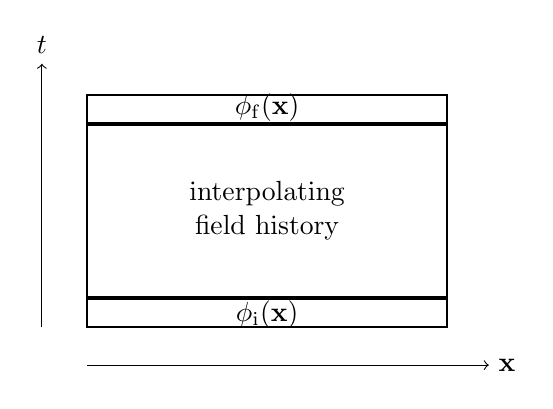
\begin{tikzpicture}[scale=0.88]
\draw[->] (-0.65,0) -- (-0.65,3.8) node[above] {$t$};
\draw[->] (0,-0.55) -- (5.8,-0.55) node[right] {$\mathbf{x}$};
\draw[thick] (0,0) rectangle (5.2,3.35);
\draw[very thick] (0,0.42) -- (5.2,0.42);
\draw[very thick] (0,2.93) -- (5.2,2.93);
\node at (2.6,0.18) {$\phi_{\mathrm{i}}(\mathbf{x})$};
\node at (2.6,3.17) {$\phi_{\mathrm{f}}(\mathbf{x})$};
\node[align=center] at (2.6,1.68) {interpolating\\field history};
\end{tikzpicture}
\caption{界定一个时空区域的初始和最终场位形。}
\end{figure}

\begin{classroomqa}
\lecturetimestamp{00:07:34}
\audiencequestion{场能回到相同的值吗？}
\lecturerresponse{能。场回到先前的值没有任何障碍，正如粒子坐标回到先前的位置没有任何障碍一样。}
\end{classroomqa}

\begin{classroomqa}
\lecturetimestamp{00:07:46}
\audiencequestion{当边界数据是场值时，为什么要谈时空事件或轨迹？}
\lecturerresponse{粒子轨迹被场的历史所取代。场空间中的每个端点都是选定时间切片上的整个场，而一段历史则指定了两个切片之间时空区域内每一点的场。}
\end{classroomqa}

要求插值场的作用量取驻值会产生偏微分方程。根据场和拉格朗日量的不同，这些方程包括麦克斯韦方程组之类，而对于引力作用量则包括爱因斯坦方程。这里不需要详细的变分推导；重要的链条是
\begin{equation}
\mathcal{L}
\longrightarrow
S[\phi]
\longrightarrow
\text{classical field equations}.
\end{equation}

\section{费曼对粒子路径的求和}

量子力学把哪条轨迹发生的问题替换为关于振幅的问题。设想在\((x,t)\)处注入一个粒子，闭眼一段时间，然后在\((x',t')\)处打开探测器。振幅
\begin{equation}
\mathcal{A}(x,t;x',t')
\end{equation}
是一个复数。其模的平方就是概率：
\begin{equation}
\begin{aligned}
P(x,t;x',t')
&=\left|\mathcal{A}(x,t;x',t')\right|^2\\
&=\mathcal{A}(x,t;x',t')
\mathcal{A}(x,t;x',t')^*.
\end{aligned}
\end{equation}

费曼规则给每一条候选路径赋予一个作用量，并与之相联系一个相位
\begin{equation}
\exp\!\left(-\frac{i}{\hbar}S[x]\right)
=
\exp\!\left[-\frac{i}{\hbar}\int \mathcal{L}(x,\dot{x})\,dt\right].
\end{equation}

\begin{figure}[htbp]
\centering
\includegraphics[width=0.70\textwidth]{lecture_10_figure_04.png}
\caption{与粒子路径相联系的复相位。}
\lectureframe{00:11:52}
\end{figure}

需要因子\(\hbar\)才能使指数无量纲。\footnote{在00:11:52处，黑板上的式子自然读作\(e^{-i\int\mathcal{L}\,dt}\)；口语中在00:12:02处补上了因子\(\hbar\)。} 跃迁振幅是这些相位对连接端点的每一条可能路径的求和：
\begin{equation}
\mathcal{A}(x,t;x',t')
=
\sum_{\substack{\text{paths }x(\tau)\\(x,t)\rightarrow(x',t')}}
\exp\!\left(-\frac{i}{\hbar}S[x]\right).
\end{equation}
这里``可能路径''并不意味着牛顿方程的解。它指的是求和中包含的任意一条路径。在非相对论量子力学中，路径沿时间向前推进，而不会向后回绕。普朗克常数具有作用的量纲，因此\(S/\hbar\)是无量纲的。

指数形式是自然的，因为相继小步的振幅相乘。若将一条路径分成连续的各段，则作用量相加，
\begin{equation}
S=S_1+S_2+\cdots,
\end{equation}
而相位相乘：
\begin{equation}
e^{-iS/\hbar}
=e^{-iS_1/\hbar}e^{-iS_2/\hbar}\cdots.
\end{equation}
因子\(i\)不是记账工具；它是量子力学规则的一部分。

\begin{classroomqa}
\lecturetimestamp{00:13:27}
\audiencequestion{指数是否与相继小步的振幅相乘有关？}
\lecturerresponse{是的。相继各步的振幅相乘，而作用量相应的各部分相加。}
\end{classroomqa}

\begin{classroomqa}
\lecturetimestamp{00:13:49}
\audiencequestion{路径求和本身是否就是概率？}
\lecturerresponse{不是。路径求和一般是复概率振幅。将它乘以其复共轭才给出概率。}
\end{classroomqa}

\section{场历史的求和}

同样的表述可以推广到量子场论，尽管这里的构造将有意保持不严格。从初始场位形\(\phi(\mathbf{x})\)和另行指定的末态场位形\(\phi'(\mathbf{x})\)出发。它们是空间的完整函数，而不是两个孤立点上的取值。

可以设想一种理想化装置，它在每个空间点上制备场，让系统演化，随后在每个点上测量场。这样的装置并不现实，但它清晰地定义了概念上的问题：从初始完整场位形过渡到末态场位形的振幅是什么？

每一种可以想象的插值场历史都有贡献。对每个历史，计算
\begin{equation}
S[\phi]=\int d^4x\,\mathcal{L}(\phi,\partial_\mu\phi)
\end{equation}
并附上相应的相位。示意地，
\begin{equation}
\mathcal{A}\!\left[\phi(\mathbf{x})\rightarrow\phi'(\mathbf{x})\right]
=
\sum_{\substack{\text{field histories}\\
\phi_{\mathrm{i}}=\phi,\;\phi_{\mathrm{f}}=\phi'}}
\exp\!\left(-\frac{i}{\hbar}S[\phi]\right).
\end{equation}
一个历史不必是经典场方程的解。它只是在中间时空区域中对场值的一种完整指定。

\begin{classroomqa}
\lecturetimestamp{00:17:39}
\audiencequestion{历史有无穷多个，而每个相位的模都是1。它们的和怎么可能收敛？这些历史是在被取极小吗？}
\lecturerresponse{这些历史是被求和，而不是被取极小。各项是分布在单位圆上的相位，因此它们可以相互抵消。这与把无穷多个远离零的正项相加不同。振荡积分可以收敛；{\proseunicodefont δ}函数的傅里叶表示就是一个熟悉的例子。如果相位均匀分布在圆周上，它们的矢量和将为零。大多数历史强烈抵消。靠近稳定作用量轨道的历史抵消得最少，因为那里的相位变化最慢，经典极限正是由此浮现。}
\end{classroomqa}

\editorialnote{实时间路径积分通常需要一种收敛规定。单位圆的讨论给出的是这里所用的振荡抵消论证，而不是收敛性的一般证明。}

这种相消可以想象为复平面中的矢量和。\footnote{单位圆的构造根据00:18:32--00:20:21的黑板讨论重新构建。}
\begin{figure}[htbp]
\centering
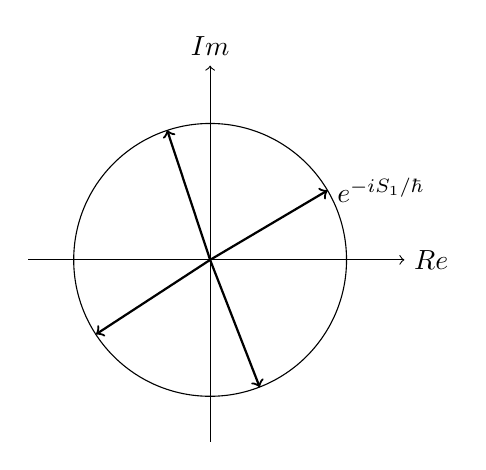
\begin{tikzpicture}[scale=1.05]
\draw[->] (-2.2,0) -- (2.35,0) node[right] {$\operatorname{Re}$};
\draw[->] (0,-2.2) -- (0,2.35) node[above] {$\operatorname{Im}$};
\draw (0,0) circle (1.65);
\draw[thick,->] (0,0) -- (1.42,0.84);
\draw[thick,->] (0,0) -- (-1.38,-0.90);
\draw[thick,->] (0,0) -- (-0.52,1.57);
\draw[thick,->] (0,0) -- (0.60,-1.54);
\node[right] at (1.42,0.84) {$e^{-iS_1/\hbar}$};
\end{tikzpicture}
\caption{当单位大小的相位方向不同时，它们可以相消。}
\end{figure}

确实，
\begin{equation}
e^{-iS/\hbar}
=
\cos\!\left(\frac{S}{\hbar}\right)
-i\sin\!\left(\frac{S}{\hbar}\right).
\end{equation}
每个贡献都是一个单位矢量。指向不同方向的贡献既相加也相减。在\(S\)的稳定点附近，邻近历史的相位几乎相同，因此它们的贡献更有效地相互增强。远离稳定作用量时，相位变化很快，相消干涉占主导。

这种路径积分结构是几乎所有现代量子场论的基础。下一步的实际做法将直接陈述而不加推导。它是进入计算的一条过度简化的途径，但它使人看到同一个对象如何能在两种语言中使用。

计算一个过程，就是计算从初态到末态的跃迁概率。一种描述指定初始场位形和最终场位形。另一种描述指定入射和出射粒子，即一个或多个场的量子。这些问题看起来不同，但二者都由同一个场论路径积分计算得出。

\section{离散时空形式}

为了使场历史求和具有具体意义，将时空划分为小单元，并为每个单元指定一个场值。通过缩小单元尺寸来趋近连续极限，但目前单元仍保持有限。这将关于函数的形式求和转化为关于给点阵单元赋数值的求和。

早先的一种启发式方法使用类似于\(1+\mathcal{L}_i\)的因子乘积，每个单元一个，然后识别描述粒子传播和碰撞的项。这一构造足够核心，值得重复，但该因子必须修正。小量不是拉格朗日量本身，而是单元内包含的作用量。

如果一个单元的时空体积为
\begin{equation}
a^4=\Delta t\,\Delta x\,\Delta y\,\Delta z,
\end{equation}
那么其作用量为
\begin{equation}
A_i=\mathcal{L}_i a^4.
\end{equation}
由于单元很小，\(A_i\)很小。暂时抑制\(\hbar\)，修正后的基本因子是
\begin{equation}
1-iA_i,
\end{equation}
而不是\(1+\mathcal{L}_i\)。

对于任意小的\(\epsilon\)，
\begin{equation}
1+\epsilon\simeq e^\epsilon,
\end{equation}
因为
\begin{equation}
e^\epsilon
=1+\epsilon+\frac{\epsilon^2}{2!}
+\frac{\epsilon^3}{3!}+\cdots.
\end{equation}
因此，在这些临时单位下，对于足够小的单元，\(1-iA_i\)近似于\(e^{-iA_i}\)。从一开始就使用精确的指数因子更为简洁。

\begin{classroomqa}
\lecturetimestamp{00:27:57}
\audiencequestion{指数是否需要\(\hbar\)因子？}
\lecturerresponse{是的。无量纲单元因子在一阶时为\(1-iA_i/\hbar\)，而精确指数为\(\exp(-iA_i/\hbar)\)。之后可以采用\(\hbar=1\)的单位。}
\end{classroomqa}

恢复\(\hbar\)后，修正的中间因子及其指数形式为
\begin{equation}
1-\frac{i}{\hbar}A_i
\simeq
\exp\!\left(-\frac{i}{\hbar}A_i\right).
\end{equation}

对于固定历史，将时空积分替换为单元作用量之和：
\begin{equation}
S[\phi]
=\int d^4x\,\mathcal{L}
\;\longrightarrow\;
\sum_i A_i.
\end{equation}
该历史的相位变为
\begin{equation}
\exp\!\left(-\frac{i}{\hbar}\sum_i A_i\right).
\end{equation}
求和的指数是指数的乘积：
\begin{equation}
\exp\!\left(-\frac{i}{\hbar}\sum_i A_i\right)
=
\prod_i\exp\!\left(-\frac{i}{\hbar}A_i\right).
\end{equation}
运算顺序很重要。首先选择一个完整历史并乘以其单元权重。只有在这之后，才对不同历史求和。

点阵也使边界数据变得明确。\footnote{棋盘及其固定的第一行和最后一行由大约00：23：54和00：30：49处的图重构。}
\begin{figure}[htbp]
\centering
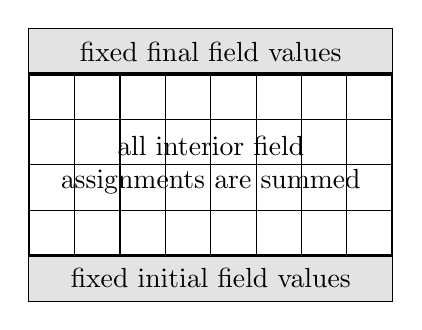
\begin{tikzpicture}[scale=0.72]
\draw[step=0.8,thin] (0,0) grid (6.4,4.8);
\draw[thick] (0,0) rectangle (6.4,4.8);
\fill[gray!22] (0,0) rectangle (6.4,0.8);
\fill[gray!22] (0,4.0) rectangle (6.4,4.8);
\draw[very thick] (0,0.8) -- (6.4,0.8);
\draw[very thick] (0,4.0) -- (6.4,4.0);
\node at (3.2,0.4) {fixed initial field values};
\node at (3.2,4.4) {fixed final field values};
\node[align=center] at (3.2,2.4) {all interior field\\assignments are summed};
\end{tikzpicture}
\caption{具有固定初始和最终点阵行的离散场历史。}
\end{figure}

第一行指定初始场位形，最后一行指定最终位形。每个内部单元允许取离散化中包含的每一个场值。因此，跃迁振幅具有如下示意形式
\begin{equation}
\mathcal{A}\!\left[\phi_{\mathrm{i}}\rightarrow\phi_{\mathrm{f}}\right]
=
\sum_{\{\phi\}_{\mathrm{interior}}}
\prod_i\exp\!\left(-\frac{i}{\hbar}A_i[\phi]\right),
\end{equation}
其中第一行和最后一行保持固定。等价地，对于每个内部赋值，计算总作用量的指数，然后将该贡献加到所有其他赋值的贡献上。

\section{从场位形到粒子位形}

同一个跃迁振幅既可以用场来描述，也可以用粒子来描述。可以不固定第一和最后一个时间切片上的场，而是指定入射的场量子集合和出射的场量子集合，然后求连接它们的振幅。被计算的对象是同一个。只有边界描述改变了。

量子场包含产生和湮灭算符。因此场的乘积通过产生、湮灭或移动量子来作用于粒子态。这种算符解读正是将点阵路径积分转化为一组粒子规则的关键。

\begin{classroomqa}
\lecturetimestamp{00:34:11}
\audiencequestion{场量子是否必然可被识别为粒子？}
\lecturerresponse{并不总是在可分别观测粒子的传统意义上如此。例如，夸克是夸克场的量子，但禁闭阻止孤立的夸克逃逸并被单独探测到。更一般地，理论中命名的场与作为传统可观测态出现的粒子种类之间不必存在一一对应。有些场论不允许这种简单对应。如果``粒子''被广义地用来指携带能量和其他量子数的不可分割的量子，那么这种区分在一定程度上可能只是术语问题。}
\end{classroomqa}

\editorialnote{源文本在00:35:45--00:36:08处的弱耦合条款在语法上存在歧义，此处不予解决。可以确定的说法是，场标签与常规可观测的粒子种类不必一一对应。}

点阵求和本身仍然遍历场的取值。它并不局限于类似光滑经典解的构型。

\begin{classroomqa}
\lecturetimestamp{00:36:44}
\audiencequestion{场的历史必须连续，或者至少近似连续吗？}
\lecturerresponse{不。在离散点阵上，相邻的元胞只是携带场的取值，而每一种赋值都被包含在求和中。并不限制于近似连续的历史。量子场涨落剧烈；典型的历史并不是光滑的经典场。}
\end{classroomqa}

被独立赋值的变量是点阵格点或元胞处的场。它们的导数由相邻取值之间的差分得到。

\begin{classroomqa}
\lecturetimestamp{00:37:56}
\audiencequestion{场及其导数是被赋予独立的值吗？}
\lecturerresponse{不。场值是在格点上被赋予的。导数随后由相邻场值之间的差分重构出来。可以采用不同的有限差分约定，但导数并不是额外的独立变量。}
\end{classroomqa}

因此，对于点阵间距\(a\)，可以示意性地写出
\begin{equation}
\partial_\mu\phi(x)
\longrightarrow
\frac{\phi(x+a\hat\mu)-\phi(x)}{a}.
\end{equation}
场值轴本身也可以被划分为小区间，从而在每个格点上留下可数多个可能取值。

\begin{classroomqa}
\lecturetimestamp{00:38:53}
\audiencequestion{当存在不止一个场时，会有什么变化？}
\lecturerresponse{在每个格点上赋予每个场的一个值，而求和遍历所有这样的赋值。}
\end{classroomqa}

复值场不应与复变量的解析函数相混淆。解析性是一种异常强的光滑性条件。场路径积分中的历史不必满足它，而且一般来说甚至不是近似光滑的。

\begin{classroomqa}
\lecturetimestamp{00:39:07}
\audiencequestion{如果场是复值的，它们的值必须满足解析函数所满足的光滑性条件吗？}
\lecturerresponse{不。复值并不意味着解析。解析函数论涉及一类极其光滑且受到严格约束的函数。这里所求和的历史不必是位置的解析函数；典型的历史高度不规则，并且在连续极限下可以被视为高度不连续的。}
\end{classroomqa}

由此得到的计算看起来令人生畏。即使在时空和场值被离散化之后，仍可能有数量极其庞大的赋值需要采样。

\begin{classroomqa}
\lecturetimestamp{00:40:04}
\audiencequestion{计算机如何知道要对多少个点阵赋值进行采样，或者计算何时已经收敛？}
\lecturerresponse{这个问题属于格点规范理论，或者更一般地说，属于格点量子场论。如今它已经是一门有效的计算学科。我参与了最初为格点规范理论建立规则的工作，而不是后来的计算机技术。建立规则花了大约三周；发展计算这些东西的技术花了大约三十年。大部分实践智慧来自统计力学，在那里配分函数也是通过对点阵构型求和得到的---例如，对晶体中某个格点是否被占据求和。判断是否已经采样了足够多的构型是一个技术问题。专家们知道---或者认为他们知道---计算何时处于可控状态，而由此得到的计算与实验相符。}
\end{classroomqa}

格点规范理论的概念性规则很快就出现了；用它们进行计算所需的技术则花了长得多的时间。棋盘格不仅仅是一个类比。它也是一种实用计算方法的起点。

\section{二次项与粒子传播}

现在回到场的算符解释。对于两个相邻格点\(x\)和\(x'\)，乘积
\begin{equation}
\phi(x)\phi(x')
\end{equation}
在适当的单粒子矩阵元中，可以提供一个格点处粒子的湮灭和另一个格点处粒子的产生。因此，在那个粒子扇区中，它可以被描绘为一次单链跃迁。这是对算符乘积的一种解读，而不是其唯一含义。

负责这类连接的是导数项。严格来说，它们并不与单个格点元胞相关联，而是与一对相邻格点相关联。例如，时间导数变为
\begin{equation}
\partial_t\phi(t,\mathbf{x})
\longrightarrow
\frac{\phi(t+a,\mathbf{x})-\phi(t,\mathbf{x})}{a},
\end{equation}
而空间导数则沿空间连线以同样的方式处理。

\begin{classroomqa}
\lecturetimestamp{00:44:39}
\audiencequestion{所讨论的拉格朗日量是否包含二阶导数？}
\lecturerresponse{这里所考虑的标准理论是用一阶导数写出的。因此它们的点阵版本使用相邻格点之间的一阶差分。}
\end{classroomqa}

对一阶差分取平方，既会产生同格点项，也会产生相邻的交叉项：
\begin{align}
\frac{1}{2}\bigl[\phi(x)-\phi(x')\bigr]^2
&=
\frac{1}{2}\phi(x)^2
+\frac{1}{2}\phi(x')^2
-\phi(x)\phi(x').
\end{align}
交叉项可以提供从一个格点到另一个格点的运动。两个平方项是同格点项。二次导数项是动能项，而正是它们的相邻交叉项将首先被用来构建传播。

为了分离出组合结构，把相邻乘积收集为
\begin{equation}
K=\sum_{\langle x,x'\rangle}\phi(x)\phi(x').
\end{equation}
路径积分权重中相应的因子示意性地写为
\begin{equation}
e^{-iK}.
\end{equation}
\editorialnote{在这个示意性的点阵因子中，点阵间距的幂次\(\hbar\)、度规符号、归一化常数以及连线的系数都被省略了。}
它的展开为
\begin{equation}
e^{-iK}
=1-iK-\frac{1}{2!}K^2+\frac{i}{3!}K^3+\cdots,
\end{equation}
或者，把相邻求和明确写出，
\begin{align}
e^{-iK}
={}&1
-i\sum_{\langle x,x'\rangle}\phi(x)\phi(x')
\nonumber\\
&-\frac{1}{2!}
\sum_{\langle x,x'\rangle}
\sum_{\langle y,y'\rangle}
\phi(x)\phi(x')\phi(y)\phi(y')
+\cdots .
\end{align}
每个因子独立地选取一对相邻格点。

粒子图遵循无悬空端点的规则。只有在边界条件明确地在初始切片上插入一个粒子或在最终切片上移除一个粒子时，才允许出现暴露的端点。内部孤立的连线具有未配对的端点，并不代表对指定跃迁的完整贡献。内部连线的端点必须相接。

首先考虑只有两个时间层的点阵。如果初态在\(x\)处插入一个粒子，而末态在相邻点\(x'\)处将其移除，那么一阶项就可以连接这两个边界插入：
\begin{equation}
x\longrightarrow x',
\qquad
\mathcal{A}_{\text{one link}}\sim -i.
\end{equation}
系数\(-i\)只是这个示意性展开中的系数；被省略的点阵因子和归一化因子仍然隐含其中。

\begin{classroomqa}
\lecturetimestamp{00:52:16}
\audiencequestion{一阶单连线项是否只在相关的初态和末态格点相邻时才贡献？}
\lecturerresponse{是的。该项选取一对相邻格点，因此只有当这些边界格点互为邻居时，它才能连接它们。更远距离的传播来自更高阶的乘积。}
\end{classroomqa}

在二阶，两个因子各自独立地对相邻格点对求和：
\begin{equation}
K^2
=
\sum_{\langle x,x'\rangle}
\sum_{\langle y,y'\rangle}
\phi(x)\phi(x')\phi(y)\phi(y').
\end{equation}

\begin{classroomqa}
\lecturetimestamp{00:52:40}
\audiencequestion{第二个相邻格点对是否必须与第一个因子所选取的格点对相邻接？}
\lecturerresponse{不。每个因子独立地选取一对相邻格点。这两对格点可以共享一个格点，可以完全分开，甚至可以就是同一对格点。求和包含每一种可能性。}
\end{classroomqa}

对于一个粒子跨越三个时间层的传播，有用的二阶选取具有一个共享的中间格点：
\begin{equation}
\bigl[\phi(x_0)\phi(x_1)\bigr]
\bigl[\phi(x_1)\phi(x_2)\bigr],
\qquad
x_0\longrightarrow x_1\longrightarrow x_2.
\end{equation}
第一条连线的末端与第二条连线的起点相接。只有\(x_0\)处的初始端点和\(x_2\)处的最终端点仍然暴露，因此该项对所要求的一粒子跃迁有贡献。在示意性指数中，它的系数为
\begin{equation}
-\frac{1}{2!}.
\end{equation}

这些选取也可以改为形成彼此分开的跳跃。\footnote{连线图是根据00：49：18--00：55：12处的序列重建的。}
\begin{figure}[htbp]
\centering
\resizebox{\linewidth}{!}{%
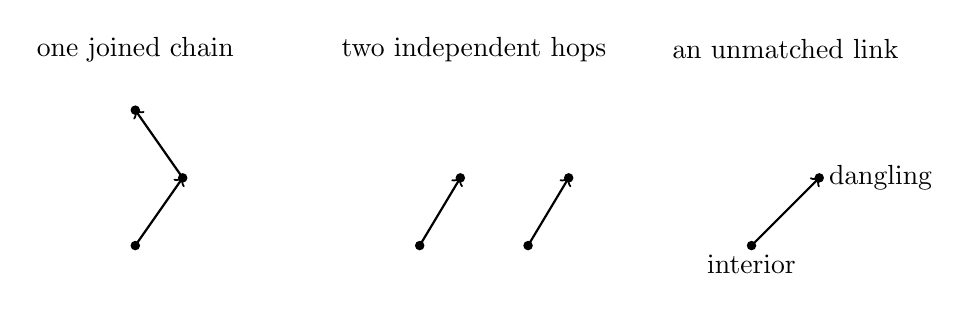
\begin{tikzpicture}[scale=0.86]
\node at (0,2.9) {one joined chain};
\fill (0,0) circle (2pt);
\fill (0.7,1.0) circle (2pt);
\fill (0,2.0) circle (2pt);
\draw[thick,->] (0,0) -- (0.7,1.0);
\draw[thick,->] (0.7,1.0) -- (0,2.0);

\begin{scope}[xshift=4.2cm]
\node at (0.8,2.9) {two independent hops};
\fill (0,0) circle (2pt);
\fill (0.6,1.0) circle (2pt);
\fill (1.6,0) circle (2pt);
\fill (2.2,1.0) circle (2pt);
\draw[thick,->] (0,0) -- (0.6,1.0);
\draw[thick,->] (1.6,0) -- (2.2,1.0);
\end{scope}

\begin{scope}[xshift=9.1cm]
\node at (0.5,2.9) {an unmatched link};
\fill (0,0) circle (2pt);
\fill (1.0,1.0) circle (2pt);
\draw[thick,->] (0,0) -- (1.0,1.0);
\node[below] at (0,0) {interior};
\node[right] at (1.0,1.0) {dangling};
\end{scope}
\end{tikzpicture}%
}
\caption{相接的、独立的以及未配对的相邻连线选取。}
\end{figure}

在这个阶数上已经可以存在不止一条路径。对于沿一个时间点阵步和一个空间点阵步的位移，以下两种顺序
\begin{align}
x
&\longrightarrow x+\hat t
\longrightarrow x+\hat t+\hat s,\\
x
&\longrightarrow x+\hat s
\longrightarrow x+\hat s+\hat t
\end{align}
到达同一个端点。

\begin{classroomqa}
\lecturetimestamp{00:55:53}
\audiencequestion{是否存在另一条两步路径到达同一个对角端点？}
\lecturerresponse{是的。可以先走时间步再走空间步，也可以按相反顺序走。两条路径都对同一个跃迁振幅有贡献。}
\end{classroomqa}

没有理由止步于两个连接。三阶项给出三个相邻连接的链。一条路径可以直接前进、绕行，或者先离开再返回，然后才到达终点。更高阶则包含更长的绕行和反复的回溯。因此，展开到任意阶就会为每一条由局部连接组装而成的路径产生一项贡献。逐点振幅就是所有这些贡献之和，其系数包含\(i\)的适当幂次和阶乘：
\begin{equation}
\begin{gathered}
\mathcal{A}(x_{\mathrm{in}}\to x_{\mathrm{out}})
=
\sum_{\text{joined lattice routes }r}c_r,
\\
c_r\ \hbox{read from the exponential expansion}.
\end{gathered}
\end{equation}
这些系数一般是复数，因此所得振幅也是复数。

相对论性传播增加了另一种可能性。一条路径可以在时间方向上既向上又向下延伸，并且可以反复经过同一条连接。

\begin{classroomqa}
\lecturetimestamp{00:58:47}
\audiencequestion{一条路径能否一遍又一遍地穿过同样的两个格点？}
\lecturerresponse{可以。重复穿越被包含在内，而且在相对论性展开中，路径还可以在时间上向后延伸。}
\end{classroomqa}

一段逆时间线段允许两种等价的图形解读。它可以被看作一条在时间中向后延伸的粒子线。或者，只沿时间向前看：一个粒子--反粒子对被产生，粒子成员继续向前，而反粒子随后与原来的粒子相遇并湮灭。同一条连通的线编码了这两种描述。\footnote{这两种解读遵循00处的图和说明：59：00--00：59：51。}

\begin{figure}[htbp]
\centering
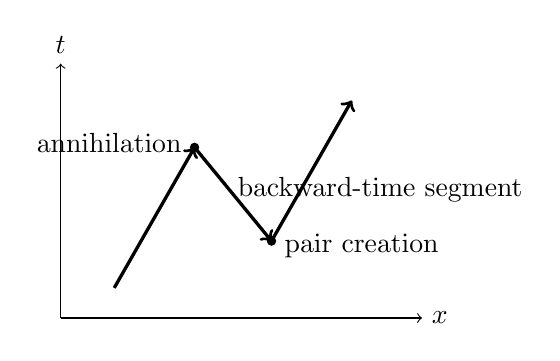
\begin{tikzpicture}[scale=0.85]
\draw[->] (0,0) -- (0,3.8) node[above] {$t$};
\draw[->] (0,0) -- (5.4,0) node[right] {$x$};
\draw[very thick,->] (0.8,0.45) -- (2.0,2.55);
\draw[very thick,->] (2.0,2.55) -- (3.15,1.15);
\draw[very thick,->] (3.15,1.15) -- (4.35,3.25);
\fill (2.0,2.55) circle (2pt);
\fill (3.15,1.15) circle (2pt);
\node[left] at (1.95,2.62) {annihilation};
\node[right] at (3.20,1.08) {pair creation};
\node[right] at (2.50,1.92) {backward-time segment};
\end{tikzpicture}
\caption{一段逆时间线段按时间向前解读为粒子对的产生和湮灭。}
\end{figure}

高阶出现的阶乘控制着指数幂级数，但这并不等同于控制对场组态的完整求和。

\begin{classroomqa}
\lecturetimestamp{01:00:00}
\audiencequestion{\(1/n!\)的因子能保证收敛吗？}
\lecturerresponse{它们保证固定自变量下指数级数的收敛。它们本身并不保证对所有场组态分别求和时的收敛。这些是不同的问题。在具有有限离散场值集合的有限点阵上，组态数目是有限的，但连续极限和无限体积极限需要进一步的控制。}
\end{classroomqa}

\section{一个连接乘积，多种粒子解读}

二阶乘积包含不止单粒子传播。当它的两个相邻对共享一个端点时，它可以使一个粒子通过一条两连接的链移动：
\begin{equation}
\bigl[\phi(x_0)\phi(x_1)\bigr]
\bigl[\phi(x_1)\phi(x_2)\bigr].
\end{equation}
当所选的对彼此分离时，同一个二阶项可以使两个粒子各移动一个连接。\footnote{单粒子传播与两次独立的单连接跳跃之间的比较，是根据01处的板书讨论重构的：00：46--01：02：34。}
\begin{equation}
\bigl[\phi(x_0)\phi(x_1)\bigr]
\bigl[\phi(y_0)\phi(y_1)\bigr],
\qquad x_0\neq y_0.
\end{equation}
第一个因子输运一个粒子，第二个因子输运另一个粒子。因此，二次点阵展开包含每个多粒子扇区中的传播振幅。同一个代数阶既可以描述一条较长的连通路径，也可以描述几条较短的非连通路径。

这包含大量信息，但它还不是真正的相互作用顶点。只有二次传播项时，连通的粒子线不会分裂成不同数目的线。改变粒子数的过程需要额外的相互作用，尽管局部算符乘积可能允许几种产生和湮灭的解读。

\begin{classroomqa}
\lecturetimestamp{01:03:30}
\audiencequestion{一个电子和一个正电子能否湮灭而不留下任何粒子？}
\lecturerresponse{一个具有非零入射能量且没有携带能量的末态的贡献违反能量守恒。当对其可能的时空位置求和时，振幅相互抵消。电子--正电子湮灭可以发生，当另一个场带走能量时---例如，当电磁量子被产生时。}
\end{classroomqa}

\editorialnote{简略的交换直接从二次跳跃跳到电子--正电子湮灭。可靠的区分在于：二次项提供自由传播，而物理湮灭需要与另一个场发生相互作用；无输出振幅因能量守恒而抵消。}

因此，导数项做了很多事，但并非全部。拉格朗日量中的进一步项由场的实验观测性质和相互作用确定。

\section{质量项}

对于标量场，所讨论的导数结构具有示意性的洛伦兹符号模式
\begin{equation}
\mathcal{L}_{\mathrm{kin}}
\sim
\frac{1}{2}\left[
(\partial_t\phi)^2
-(\partial_x\phi)^2
-(\partial_y\phi)^2
-(\partial_z\phi)^2
\right].
\end{equation}
该式固定了与讨论相关的时间减空间结构；整体符号与归一化约定则保持隐含。

拉格朗日量也可以包含未微分场的幂次。二次项的例子具有如下形式
\begin{equation}
\text{mass term}\ \propto\ \frac{1}{2}m^2\phi^2,
\end{equation}
其中\(m^2\)被认定为质量系数。\editorialnote{本段来源并未固定完整标量拉格朗日量的整体符号约定。}在示意性的粒子解读中，这一项湮灭一个粒子并在同一格点上重新产生它。它并不移动粒子。它向路径中插入一个同格点因子：
\begin{equation}
\text{particle at }x
\longrightarrow
\boxed{m^2\phi(x)^2}
\longrightarrow
\text{particle still at }x.
\end{equation}
每当这样的插入作用一次，路径就获得另一个正比于\(m^2\)的因子。

如果只保留导数项，则在这一示意性展开中得到的传播是无质量理论。对于有质量场，一条路径可以在其跳跃项之间包含任意数量的同格点质量插入。质量项改变各路径的相对权重，使得最终得到的传播子携带粒子的质量。

\section{三次项与分裂--重新合并历史}

质量项改变路径的权重而不移动粒子。更有趣的行为始于次数高于二次的项。取一个三次相互作用，
\begin{equation}
\mathcal{L}_{\mathrm{int}}=g_3\phi^3.
\end{equation}
在一个格胞上，三个场因子有四种粒子解读：
\begin{equation}
1\longrightarrow 2,
\qquad
2\longrightarrow 1,
\qquad
0\longrightarrow 3,
\qquad
3\longrightarrow 0.
\end{equation}
因此一个三次因子可以湮灭一个粒子并产生两个，湮灭两个并产生一个，产生三个，或湮灭三个。

二次的相邻对因子仍然提供传播。一串这样的因子可以把一个粒子带到某个格胞，该格胞处的一个三次因子可以吸收它并发射两个粒子，而进一步的二次因子可以把这两个粒子带走。这为一个具有一个入射粒子和两个出射粒子的振幅作出贡献。\footnote{点阵几何由01处的图重构：08：48--01：09：42。}

\begin{figure}[htbp]
\centering
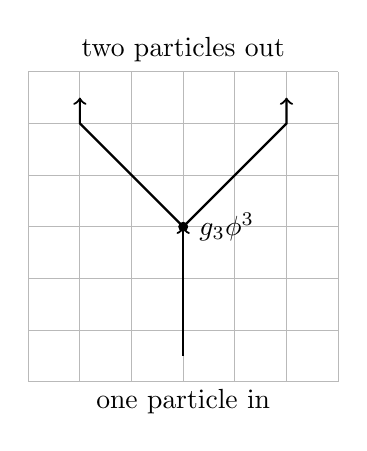
\begin{tikzpicture}[scale=0.82]
\draw[step=0.8,gray!55,thin] (0,0) grid (4.8,4.8);
\draw[thick,->] (2.4,0.4) -- (2.4,1.2) -- (2.4,2.0) -- (2.4,2.4);
\fill (2.4,2.4) circle (2.2pt);
\draw[thick,->] (2.4,2.4) -- (1.6,3.2) -- (0.8,4.0) -- (0.8,4.4);
\draw[thick,->] (2.4,2.4) -- (3.2,3.2) -- (4.0,4.0) -- (4.0,4.4);
\node[right] at (2.5,2.4) {$g_3\phi^3$};
\node at (2.4,-0.3) {one particle in};
\node at (2.4,5.15) {two particles out};
\end{tikzpicture}
\caption{二次因子将一个粒子传播进入并离开一个三次分裂顶点。}
\end{figure}

即便是一个初态和末态都只有一个粒子的振幅，也不再仅仅是一串单一不间断路径之和。一个贡献是由一串二次跳跃直接传播。另一个贡献包含两个三次因子：粒子分裂成两个，而这两个后来重新合并。因此中间态可以包含比外态更多的粒子。\footnote{这两种备选情形由01处的图重构：09：44--01：11：36。}

\begin{figure}[htbp]
\centering
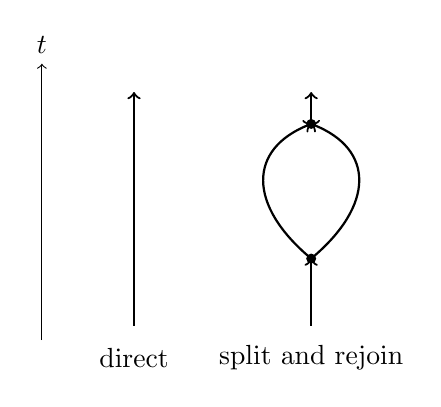
\begin{tikzpicture}[scale=0.9]
\draw[->] (-0.7,0) -- (-0.7,3.9) node[above] {$t$};
\draw[thick,->] (0.6,0.2) -- (0.6,3.5);
\node at (0.6,-0.25) {direct};
\draw[thick,->] (3.1,0.2) -- (3.1,1.15);
\fill (3.1,1.15) circle (2pt);
\draw[thick,->] (3.1,1.15) .. controls (2.2,1.9) and (2.2,2.7) .. (3.1,3.05);
\draw[thick,->] (3.1,1.15) .. controls (4.0,1.9) and (4.0,2.7) .. (3.1,3.05);
\fill (3.1,3.05) circle (2pt);
\draw[thick,->] (3.1,3.05) -- (3.1,3.5);
\node at (3.1,-0.25) {split and rejoin};
\end{tikzpicture}
\caption{对同一个单粒子振幅的直接传播与分裂--重新合并贡献。}
\end{figure}

在电动力学中，相应的例子是一个电子发射一个光子，随后又将其重新吸收。这一发射并重新吸收的历史是电子从一点传播到另一点的振幅的一部分。更高阶包含若干次发射和吸收。一个光子可以转化为一个电子--正电子对，而该中间对中的电子和正电子本身又可以交换一个光子。仅仅因为初态和末态的粒子内容简单，并不要求中间粒子内容看起来也简单。\footnote{以下重构中的例子出现在01：11：22--01：12：34。}

\begin{figure}[htbp]
\centering
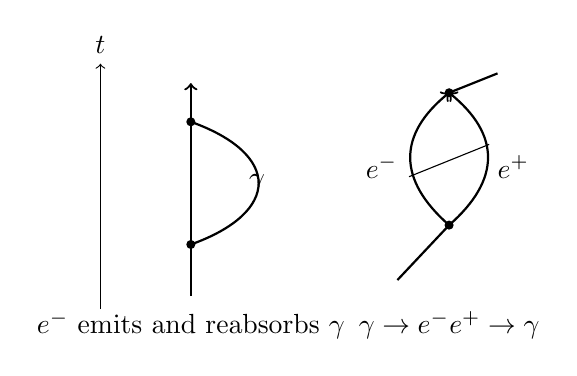
\begin{tikzpicture}[scale=0.82]
\draw[->] (-0.6,0) -- (-0.6,3.8) node[above] {$t$};
\draw[thick,->] (0.8,0.2) -- (0.8,3.5);
\fill (0.8,1.0) circle (2pt);
\fill (0.8,2.9) circle (2pt);
\draw[thick] (0.8,1.0) .. controls (2.2,1.5) and (2.2,2.4) .. (0.8,2.9);
\node[right] at (1.55,1.95) {$\gamma$};
\node at (0.8,-0.25) {$e^-$ emits and reabsorbs $\gamma$};
\draw[thick] (4.0,0.45) -- (4.8,1.3);
\fill (4.8,1.3) circle (2pt);
\draw[thick,->] (4.8,1.3) .. controls (4.0,2.0) and (4.0,2.7) .. (4.8,3.35);
\draw[thick,->] (4.8,1.3) .. controls (5.6,2.0) and (5.6,2.7) .. (4.8,3.35);
\fill (4.8,3.35) circle (2pt);
\draw[thick] (4.8,3.35) -- (5.55,3.65);
\draw[thin] (4.18,2.05) -- (5.42,2.55);
\node[left] at (4.15,2.2) {$e^-$};
\node[right] at (5.4,2.2) {$e^+$};
\node at (4.8,-0.25) {$\gamma\to e^-e^+\to\gamma$};
\end{tikzpicture}
\caption{一个电子自发射贡献，以及一个包含电子--正电子对的光子历史。}
\end{figure}

每一条这样的历史都来自指数展开中各项的一个确定乘积。其系数携带适当的\(i\)的幂、来自指数级数的一个阶乘，以及附着在其顶点上的耦合常数。该系数给出那条历史的贡献，但对于指定初态和末态的振幅，是具有相同外态的所有历史之和。

\begin{classroomqa}
\lecturetimestamp{01:13:18}
\audiencequestion{同一个整体过程能否以若干不同的历史发生，从而使它们全都对其振幅作出贡献？}
\lecturerresponse{能。该过程的振幅由把同一初态连接到同一末态的所有不同历史得到。}
\end{classroomqa}

因此，组织量子场论有两种等价的方式。在场描述中，人们指定初始场位形和最终场位形，并对介于其间的每一个场历史求和。在粒子描述中，场被分解为量子：人们指定入射粒子内容和出射粒子内容，并对连接它们的全部粒子历史求和。同一个拉格朗日量支配着这两种描述。

\section{四次项、守恒定律与耦合}

四次相互作用
\begin{equation}
\mathcal{L}_{\mathrm{int}}=g_4\phi^4,
\end{equation}
在同一点有四个场因子。它的局域粒子读法包括
\begin{equation}
\begin{gathered}
2\longrightarrow2,
\qquad
1\longrightarrow3,
\qquad
3\longrightarrow1,\\
0\longrightarrow4,
\qquad
4\longrightarrow0.
\end{gathered}
\end{equation}
因此，一个四腿顶点可以描述两粒子散射、一个粒子分裂为三个、三个合并为一个，或者四条腿全部朝外或全部朝内。\footnote{这些朝向由图01：14：28--01：15：18重构。}

\begin{figure}[htbp]
\centering
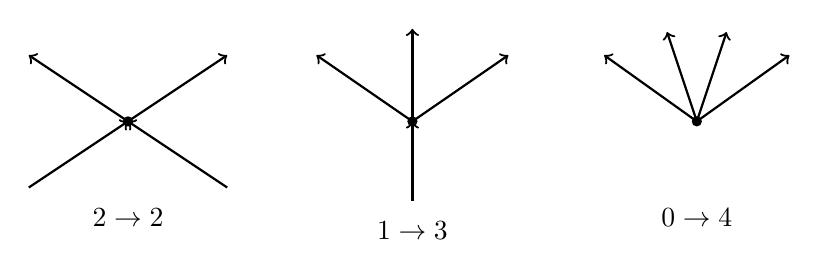
\begin{tikzpicture}[scale=0.84]
\fill (0,0) circle (2.2pt);
\draw[thick,->] (-1.5,-1.0) -- (0,0);
\draw[thick,->] (1.5,-1.0) -- (0,0);
\draw[thick,->] (0,0) -- (-1.5,1.0);
\draw[thick,->] (0,0) -- (1.5,1.0);
\node at (0,-1.45) {$2\to2$};
\begin{scope}[xshift=4.3cm]
\fill (0,0) circle (2.2pt);
\draw[thick,->] (0,-1.2) -- (0,0);
\draw[thick,->] (0,0) -- (-1.45,1.0);
\draw[thick,->] (0,0) -- (0,1.4);
\draw[thick,->] (0,0) -- (1.45,1.0);
\node at (0,-1.65) {$1\to3$};
\end{scope}
\begin{scope}[xshift=8.6cm]
\fill (0,0) circle (2.2pt);
\draw[thick,->] (0,0) -- (-1.4,1.0);
\draw[thick,->] (0,0) -- (-0.45,1.35);
\draw[thick,->] (0,0) -- (0.45,1.35);
\draw[thick,->] (0,0) -- (1.4,1.0);
\node at (0,-1.45) {$0\to4$};
\end{scope}
\end{tikzpicture}
\caption{四腿相互作用顶点的三种局域朝向。}
\end{figure}

局域读法\(0\to4\)本身并不说明四个粒子可以作为一个物理过程从真空中出现。这个顶点仍然必须对每一个可能的时空位置求和。当所提出的外部态不能守恒能量时，来自这些位置的相位会相消。

\begin{classroomqa}
\lecturetimestamp{01:15:18}
\audiencequestion{四出朝向描述的是四个粒子自发地出现在末态中吗？}
\lecturerresponse{它是四场算符的一种局域读法，但一个没有入射能量的过程违反能量守恒。当把来自顶点所有可能时空位置的振幅相加时，它们相消为零。}
\end{classroomqa}

\begin{classroomqa}
\lecturetimestamp{01:15:58}
\audiencequestion{能量守恒和动量守恒是从计算本身中涌现出来的吗？}
\lecturerresponse{是的。对顶点在所有时间上积分会强制能量守恒，在所有空间上积分会强制动量守恒。除非两者都守恒，否则对顶点位置的求和为零。}
\end{classroomqa}

在这些守恒定律的约束下，拉格朗日量所允许的每一个图都贡献一定的振幅。该贡献的大小部分取决于每个相互作用项的系数。把三次和四次系数写作\(G_3\)和\(G_4\)。每一个三腿顶点贡献一个\(G_3\)因子，每一个四腿顶点贡献一个\(G_4\)因子。因此，一个具有\(V_3\)个三次顶点和\(V_4\)个四次顶点的图，其耦合依赖关系的示意形式为
\begin{equation}
\mathcal{A}_{\mathrm{graph}}
\propto G_3^{V_3}G_4^{V_4}.
\end{equation}

如果这些耦合很小，那么顶点少的图一般比顶点多的图贡献更大。每增加一个顶点就带来另一个小因子。这使微扰求和有机会变得有用：从最简单的图开始，然后依次加入越来越小的修正。

完整级数是否真正收敛是一个困难的问题。小耦合使这种排序看似合理，但它们本身并不能解决所有收敛问题。在大耦合下，朴素的级数可能完全失效。这种失效并不表明底层理论是错的；它可能只表明按耦合的幂展开是一种糟糕的计算方式。所讨论的方法最直接有用的时候，是耦合小到具有四个顶点的图远小于具有两个顶点的图。

\begin{classroomqa}
\lecturetimestamp{01:19:24}
\audiencequestion{色理论可以用同样的方式处理吗？}
\lecturerresponse{可以。色理论可以用同样的方式表述，并将在后面讨论。}
\end{classroomqa}

\section{传播子、顶点与互补描述}

下一个任务是列出粒子，并把它们的动力学要么编码在拉格朗日量中，要么编码在费曼规则中。这是同一信息的两种形式。二次项描述从一点到另一点的传播。表示这种传播的线称为传播子。涉及三个或更多场的项描述线相交的地方。那些相交点就是顶点。例如，
\begin{equation}
\begin{aligned}
\text{quadratic term}
&\longleftrightarrow \text{propagator},\\
G_3\phi^3
&\longleftrightarrow \text{three-leg vertex}.
\end{aligned}
\end{equation}

人们可以通过为每个粒子给出一个量子场，并写出一个包含它们所有质量和相互作用的拉格朗日量来指定一个理论。等价地，人们可以列出每一个传播子、每一个允许的顶点，以及附着在每个顶点上的系数。无论哪一种清单都告诉我们哪些过程是可能的，以及如何为它们的图指定振幅。

例如，两个电子可以通过交换一个光子而散射。每条电子线包含一个电子--电子--光子顶点，而光子传播子连接这两个顶点。\footnote{该图由01中的例子重构而来：21：38。}

\begin{figure}[htbp]
\centering
\begin{tikzpicture}[scale=0.95]
\draw[->] (-0.6,-0.2) -- (0.2,1.4);
\draw[->] (0.2,1.4) -- (-0.7,3.1);
\draw[->] (3.5,-0.2) -- (2.7,1.4);
\draw[->] (2.7,1.4) -- (3.6,3.1);
\fill (0.2,1.4) circle (2pt);
\fill (2.7,1.4) circle (2pt);
\draw[thick] (0.2,1.4) -- (2.7,1.4);
\node[above] at (1.45,1.4) {$\gamma$};
\node[left] at (-0.2,0.5) {$e^-$};
\node[right] at (3.1,0.5) {$e^-$};
\end{tikzpicture}
\caption{通过交换一个光子进行的双电子散射。}
\end{figure}

拉格朗日量决定了该图的振幅，并包含约束它的对称性和守恒定律。在时间取向的图中，位于底部的粒子构成初态位形，位于顶部的粒子构成末态位形。

\begin{classroomqa}
\lecturetimestamp{01:22:06}
\audiencequestion{在费曼图中，底部的粒子是初态位形，顶部的粒子是末态位形吗？}
\lecturerresponse{是的。底部是初始粒子位形，顶部是最终粒子位形。}
\end{classroomqa}

粒子描述与场描述是互补的，正如在普通量子力学中动量和位置是互补的描述一样。它们以不同的基描述同一个系统。也存在相应的不确定性：如果粒子数被精确指定，则场值不确定；如果场值被精确指定，则粒子数不确定。两种描述都不能取代另一种，而拉格朗日量在两者中都很有用。

\begin{classroomqa}
\lecturetimestamp{01:23:26}
\audiencequestion{耦合常数是由理论预言的，还是由实验确定的？}
\lecturerresponse{对称性有时可以将一个耦合常数与另一个联系起来，但它们的数值一般来自实验。}
\end{classroomqa}

\section{测量输入与广泛预言}

量子场论本身具有优雅和美感。但当人们开始列举事实---有哪些粒子、它们的质量是多少、它们的耦合常数是多少---时，这份清单却是一团乱麻。它是一团非常丑陋的乱麻，除了对称性所提供的连贯性之外几乎没有连贯性。对称性将不同种类的粒子及其过程联系起来，但只在有限的程度上。清单中的大部分内容仍然是一大堆关于某种缺乏动机的不同种类粒子的、相对随机的事实。

\begin{classroomqa}
\lecturetimestamp{01:24:58}
\audiencequestion{为什么测量得到的耦合常数应当被如此自信地信任？}
\lecturerresponse{一旦某个耦合被测量，改变它就会给出错误的预言。它的数值由许多使用它的计算来检验。}
\end{classroomqa}

粒子太多了，这意味着场太多了---多到任何审美感都无法接受。大约有一百种左右。耦合常数很多，或多或少是从实验中得来的数字，质量也很多，而且分布范围很广。它们之间有一些关系，但只有少数几个。

但一旦知道了它们，你就可以开始计算。一旦知道了它们，就是这样：人们可以极其精确地计算关于这些粒子的任何事情。关于夸克、电子、光子以及其他一切的任何事情，都延伸到原子物理、粒子物理、核物理、化学，也许还有生物学。输入的量可能比人们希望的要多，但输出的量是巨大的。

\section{量子电动力学作为微扰示例}

量子电动力学给出了耦合展开的一个具体例子。

\begin{classroomqa}
\lecturetimestamp{01:26:12}
\audiencequestion{对于电子和光子，\(G_n\)类型的相互作用耦合有多少个？}
\lecturerresponse{有一个基本相互作用耦合：电荷\(e\)。它是一个\(G_3\)类型的系数，附着在一个顶点上，该顶点有一个电子进入、一个电子离开，以及一个光子被发射或吸收。}
\end{classroomqa}

忽略旋量矩阵和指标，该相互作用具有如下示意性的场内容
\begin{equation}
\mathcal{L}_{\mathrm{QED,int}}
\sim e\,(\text{electron bilinear})\,A,
\end{equation}
其中\(A\)表示光子场。对于计数论证而言，详细的狄拉克矩阵结构并不需要。量子电动力学的基本规则是电子发射或吸收一个光子；所有更复杂的量子电动力学图都由反复使用这一个顶点组装而成。\footnote{该示意性顶点由01重构而来：26：42；详细的矩阵结构在原始材料中被有意忽略。}

\begin{figure}[htbp]
\centering
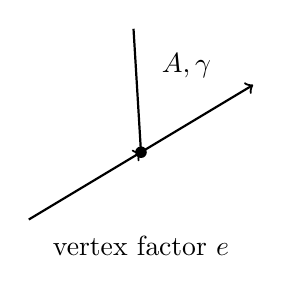
\begin{tikzpicture}[scale=0.95]
\draw[thick,->] (-1.5,-0.9) -- (0,0);
\draw[thick,->] (0,0) -- (1.5,0.9);
\draw[thick] (0,0) -- (-0.1,1.65);
\fill (0,0) circle (2.2pt);
\node[right] at (0.15,1.15) {$A,\gamma$};
\node at (0,-1.25) {vertex factor $e$};
\end{tikzpicture}
\caption{量子电动力学的基本电子--电子--光子顶点。}
\end{figure}

\begin{classroomqa}
\lecturetimestamp{01:27:38}
\audiencequestion{电子--质子散射呢？}
\lecturerresponse{在初等的原子处理中，质子可以理想化为一个固定、无限重的点源---——一个被钉在原处的重粒子。它自身的量子场动力学只有在把质子和中子的内部理论纳入进来时才起作用。}
\end{classroomqa}

\begin{classroomqa}
\lecturetimestamp{01:28:30}
\audiencequestion{电子能否相对于那个质子以接近光速的速度运动？}
\lecturerresponse{能。}
\end{classroomqa}

考虑光子被电子散射。在最低阶，该图有两个电子--电子--光子顶点。因此振幅正比于\(e^2\)：
\begin{equation}
\mathcal{A}_{\mathrm{lowest}}\propto e^2.
\end{equation}
概率，或者等价地说，截面与耦合的依赖关系，来自绝对值的平方，正比于\(e^4\)：
\begin{equation}
P_{\mathrm{lowest}}\ \text{or}\ \sigma_{\mathrm{lowest}}
\propto e^4.
\end{equation}
在通常的无量纲归一化下，电耦合很小，因此真正的散射比光子径直穿过而不发生散射的可能性要小得多。

在这一阶已经有两个图。在一种时间顺序中，入射光子先被吸收，出射光子稍后被发射。在另一种中，出射光子在入射光子被吸收之前先被发射。两个振幅都有贡献。\footnote{这两种时间顺序可由01：28：42和01：30：18处的图重构出来。}

\begin{figure}[htbp]
\centering
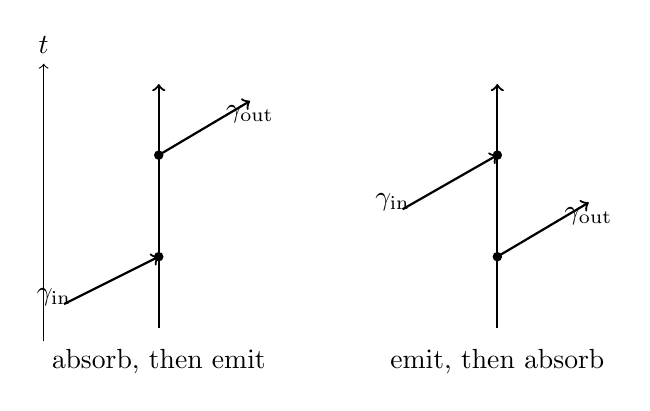
\begin{tikzpicture}[scale=0.86]
\draw[->] (-0.7,0) -- (-0.7,4.1) node[above] {$t$};
\draw[thick,->] (1.0,0.2) -- (1.0,3.8);
\fill (1.0,1.25) circle (2pt);
\fill (1.0,2.75) circle (2pt);
\draw[thick,->] (-0.4,0.55) -- (1.0,1.25);
\draw[thick,->] (1.0,2.75) -- (2.35,3.55);
\node[left] at (-0.15,0.65) {$\gamma_{\mathrm{in}}$};
\node[right] at (1.85,3.35) {$\gamma_{\mathrm{out}}$};
\node at (1.0,-0.3) {absorb, then emit};
\begin{scope}[xshift=5.0cm]
\draw[thick,->] (1.0,0.2) -- (1.0,3.8);
\fill (1.0,1.25) circle (2pt);
\fill (1.0,2.75) circle (2pt);
\draw[thick,->] (1.0,1.25) -- (2.35,2.05);
\draw[thick,->] (-0.4,1.95) -- (1.0,2.75);
\node[right] at (1.85,1.85) {$\gamma_{\mathrm{out}}$};
\node[left] at (-0.15,2.05) {$\gamma_{\mathrm{in}}$};
\node at (1.0,-0.3) {emit, then absorb};
\end{scope}
\end{tikzpicture}
\caption{电子--光子散射的两个最低阶时间顺序。}
\end{figure}

因此最低阶振幅不是一个图，而是两者之和：
\begin{equation}
\begin{aligned}
\mathcal{A}^{(2)}
&=
\mathcal{A}_{\mathrm{absorb\ then\ emit}}
+\mathcal{A}_{\mathrm{emit\ then\ absorb}},\\
\mathcal{A}^{(2)}&\propto e^2.
\end{aligned}
\end{equation}

更高阶修正会加入更多基本顶点。一个额外内线光子两次附着在电子线上，会加入两个\(e\)因子，在振幅中给出正比于\(e^4\)的贡献，在其模平方中给出正比于\(e^8\)的贡献。一条光子线也可以包含一个电子--正电子插入，同样加入基本顶点和额外的\(e\)幂次。这些只是例子，并非穷尽列表；额外光子可以附着在许多位置上。\footnote{更高阶结构可由01：30：38--01：31：16重构出来。}

\begin{figure}[htbp]
\centering
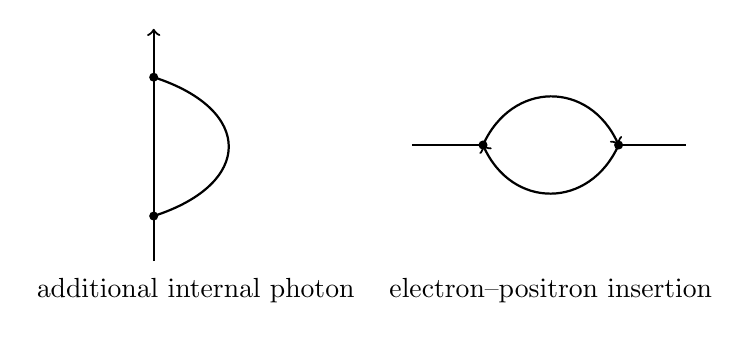
\begin{tikzpicture}[scale=0.82]
\draw[thick,->] (0.9,0.2) -- (0.9,3.8);
\fill (0.9,0.9) circle (2pt);
\fill (0.9,3.05) circle (2pt);
\draw[thick] (0.9,0.9) .. controls (2.45,1.4) and (2.45,2.55) .. (0.9,3.05);
\node at (1.55,-0.25) {additional internal photon};
\begin{scope}[xshift=5.1cm]
\draw[thick] (-0.2,2.0) -- (0.9,2.0);
\fill (0.9,2.0) circle (2pt);
\fill (3.0,2.0) circle (2pt);
\draw[thick,->] (0.9,2.0) .. controls (1.35,3.0) and (2.55,3.0) .. (3.0,2.0);
\draw[thick,->] (3.0,2.0) .. controls (2.55,1.0) and (1.35,1.0) .. (0.9,2.0);
\draw[thick] (3.0,2.0) -- (4.05,2.0);
\node at (1.95,-0.25) {electron--positron insertion};
\end{scope}
\end{tikzpicture}
\caption{两个更高阶的QED结构，它们加入基本顶点和额外的\(e\)幂次。}
\end{figure}

因此QED展开按\(e^2\)的逐次幂进行。每一个相当的新复杂化都会在振幅中加入两个电荷的幂次。在所使用的归一化下，这使得此类修正在振幅上比前一阶大约小一百倍或两百倍。更复杂的图逐渐更弱，因此微扰求和有机会变得有用。

概率并不是通过分别对每个图平方、再把这些平方相加得到的。首先要把对同一外部过程有贡献的每个振幅相加：
\begin{equation}
\mathcal{A}_{\mathrm{total}}=\sum_r\mathcal{A}_r.
\end{equation}
然后才构成
\begin{equation}
P=\left|\mathcal{A}_{\mathrm{total}}\right|^2
=\left|\sum_r\mathcal{A}_r\right|^2.
\end{equation}
不同图之间的交叉项是干涉项。规则简单而本质：先相加，再平方。

\section{走向粒子清单与标准模型}

有了传播子、顶点、耦合计数和干涉，粒子物理的描述就可以正式开始了。人们可以命名粒子，指定它们的质量，写出部分来自理论、部分来自实验的支配它们的拉格朗日量，并直接在这些拉格朗日量中研究它们的对称性。同一框架随后导向标准模型及其性质。

\begin{classroomqa}
\lecturetimestamp{01:33:22}
\audiencequestion{常数质量系数\(m^2\)能否被希格斯场取代？}
\lecturerresponse{能。这正是正确的想法，该机制将在后面讨论。}
\end{classroomqa}

\begin{classroomqa}
\lecturetimestamp{01:33:42}
\audiencequestion{相邻点阵点\(x\)和\(x'\)能否位于两个不同的时刻？}
\lecturerresponse{能。它们可以是时间方向上的相邻点；点阵上的竖直传播就是这样表示的。}
\end{classroomqa}

对于相邻点，有限差分平方同时包含同点项和跨链项：
\begin{equation}
\bigl[\phi(x)-\phi(x')\bigr]^2
=
\phi(x)^2+\phi(x')^2-2\phi(x)\phi(x').
\end{equation}

\begin{classroomqa}
\lecturetimestamp{01:33:56}
\audiencequestion{哪一项表示粒子只是静止不动？}
\lecturerresponse{有限差分平方中的同点项\(\phi(x)^2\)和\(\phi(x')^2\)表示静止不动，而交叉项\(\phi(x)\phi(x')\)提供运动的解释。显式质量项也贡献同点、静止不动的因子。}
\end{classroomqa}
